% !TeX root = ../main.tex

\chapter{Modelos de ecuaciones diferenciales difusos}
La construcción de los capítulos anteriores ha tenido como uno de sus objetivos principales la aplicación de las teorías expuestas a la realidad. Es por ello, que en este capítulo se analizará el potencial y la exactitud de estos métodos para modelar la realidad al añadir una serie de constantes difusas.

Se verá, como ejemplo, que sucede cuando se tiene en cuenta la incertidumbre estándar como números difusos.

\section{Aplicaciones a las ciencias naturales}

En esta sección vamos a ver modelos matemáticos donde aparecen la incertidumbre de manera natural al tener en cuenta constantes físicas o errores de medidas. 

Se puede observar en \cite{nasa} los errores que se cometen al usar una serie de constantes astronómicas, este hecho será interesante para plantear una serie de problemas.
\subsection{Aplicaciones a la mecánica clásica}
En primer lugar, se resolverá un problema básico de propulsión de un cohete teniendo en cuenta el error de medidas en los aparatos del cohete.
\subsubsection{Propulsión de un cohete}

\begin{ejemplo}[\cite{Giancoli}]
	Un cohete lleno de combustible tiene una masa aproximadamente de $21000kg$ de los cuales $15000kg$ aproximadamente son de combustible, por simplificar, se supone que son medidas exactas.
\end{ejemplo}
Por otro lado, se va a plantear es la órbita de un planeta de manera clásica teniendo en cuenta ahora las constantes y su incertidumbre

\subsubsection{Orbita planetaria}
\begin{ejemplo}
	Se trata de encontrar la posición respecto al sol de un planeta en un tiempo $t$, para resolver este problema se usará \textit{Ley de la Gravitación Universal} que dice:
	\[
	F_G = \frac{GM m}{r^2}
	\]
	Donde $G=6.67424 \times 10^{-11} \pm 6.7 \times 10^{-15} m^3 kg^{-1} s^{-2}$ y $M$ es la masa del sol, que en este caso, $M=1.9884\times 10^{30} \pm 2 \times 10^{26} kg$, debido a la naturaleza de estas constantes podemos expresarlas como números triangulares, y de esta forma se convierte el problema clásico en un problema difuso.
	
	Por otro lado, se puede expresar $r$ como la distancia al sol, y dado que el sol se ha tomado como punto de referencia, $r=\sqrt{x^2+y^2}$ donde $x, y$ son las posiciones respecto a los eje $x, y$ respectivamente.
	
	En otro orden de cosas, si se aplica la segunda ley de Newton, se sabe que $\vec{F} = m \vec{a}$, por tanto se puede escribir la aceleración dada por la gravedad como 
	\[
	\vec{a} = -\frac{GM}{r^2} \left(
	\cos{\sigma}, \sin{\sigma}
	\right)
	\]
	Y teniendo en cuenta la definición de seno, y coseno se puede escribir finalmente:
	\[
	\begin{array}{l||r}
	a_x = - \frac{GMx}{r^3} & a_y = - \frac{GMy}{r^3}
	\end{array}
	\]
	
	Y dado que por definición la aceleración es la segunda derivada de la ecuación de posición respecto al tiempo, se tiene:
	\[
	\vec{a} = \frac{d\vec{s}}{dt}
	\]
	
	Se definen ahora los números triangulares $G=(6.67357\times10^{-11};6.67424 \times 10^{-11};6.67491\times10^{-11})$ y $M=(1.9882\times10^{30};1.9884\times 10^{30}
	;1.9886\times10^{30})$, se puede definir $I=G\cdot M$.
	
	
	\begin{figure}[h]
		\centering
		\begin{subfigure}[b]{0.49\textwidth}
			\frame{
				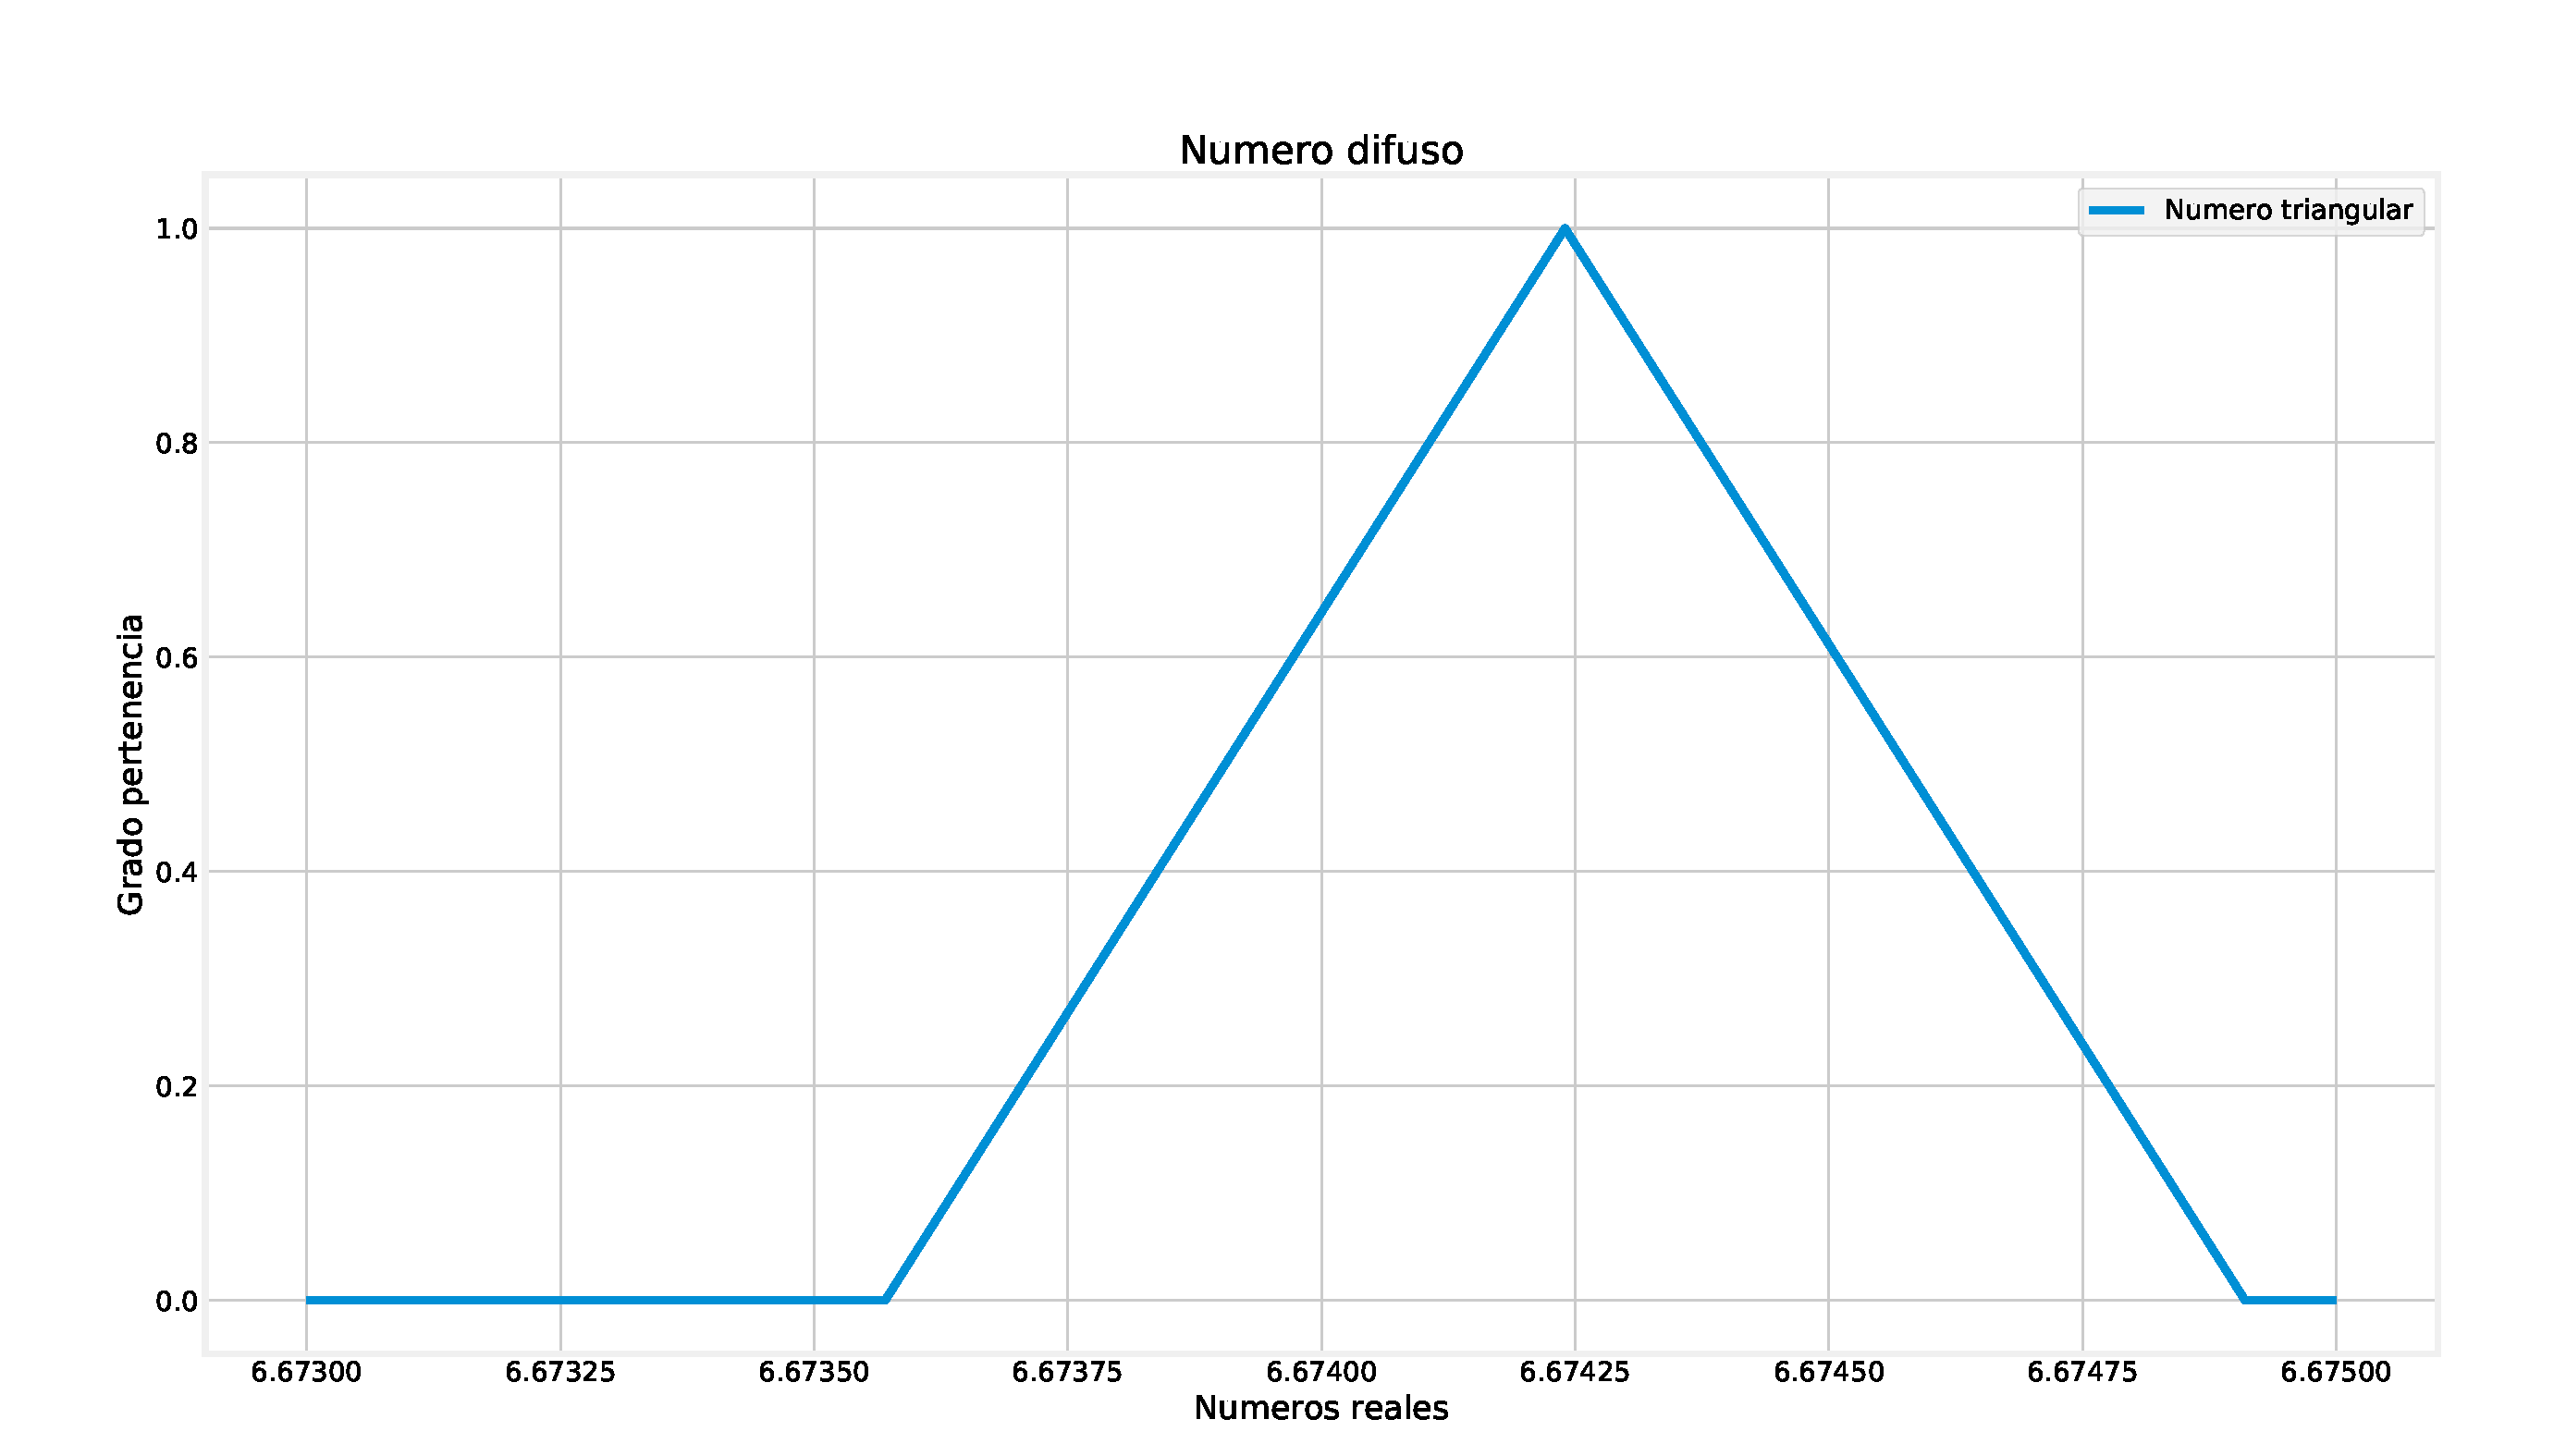
\includegraphics[width=\textwidth]{grafica_triangular_orbita_g.pdf}}
			\caption{Gráfica del número difuso $G$}
			\label{fig:triangular_g}
		\end{subfigure}
		~ 
		\begin{subfigure}[b]{0.49\textwidth}
			\frame{
				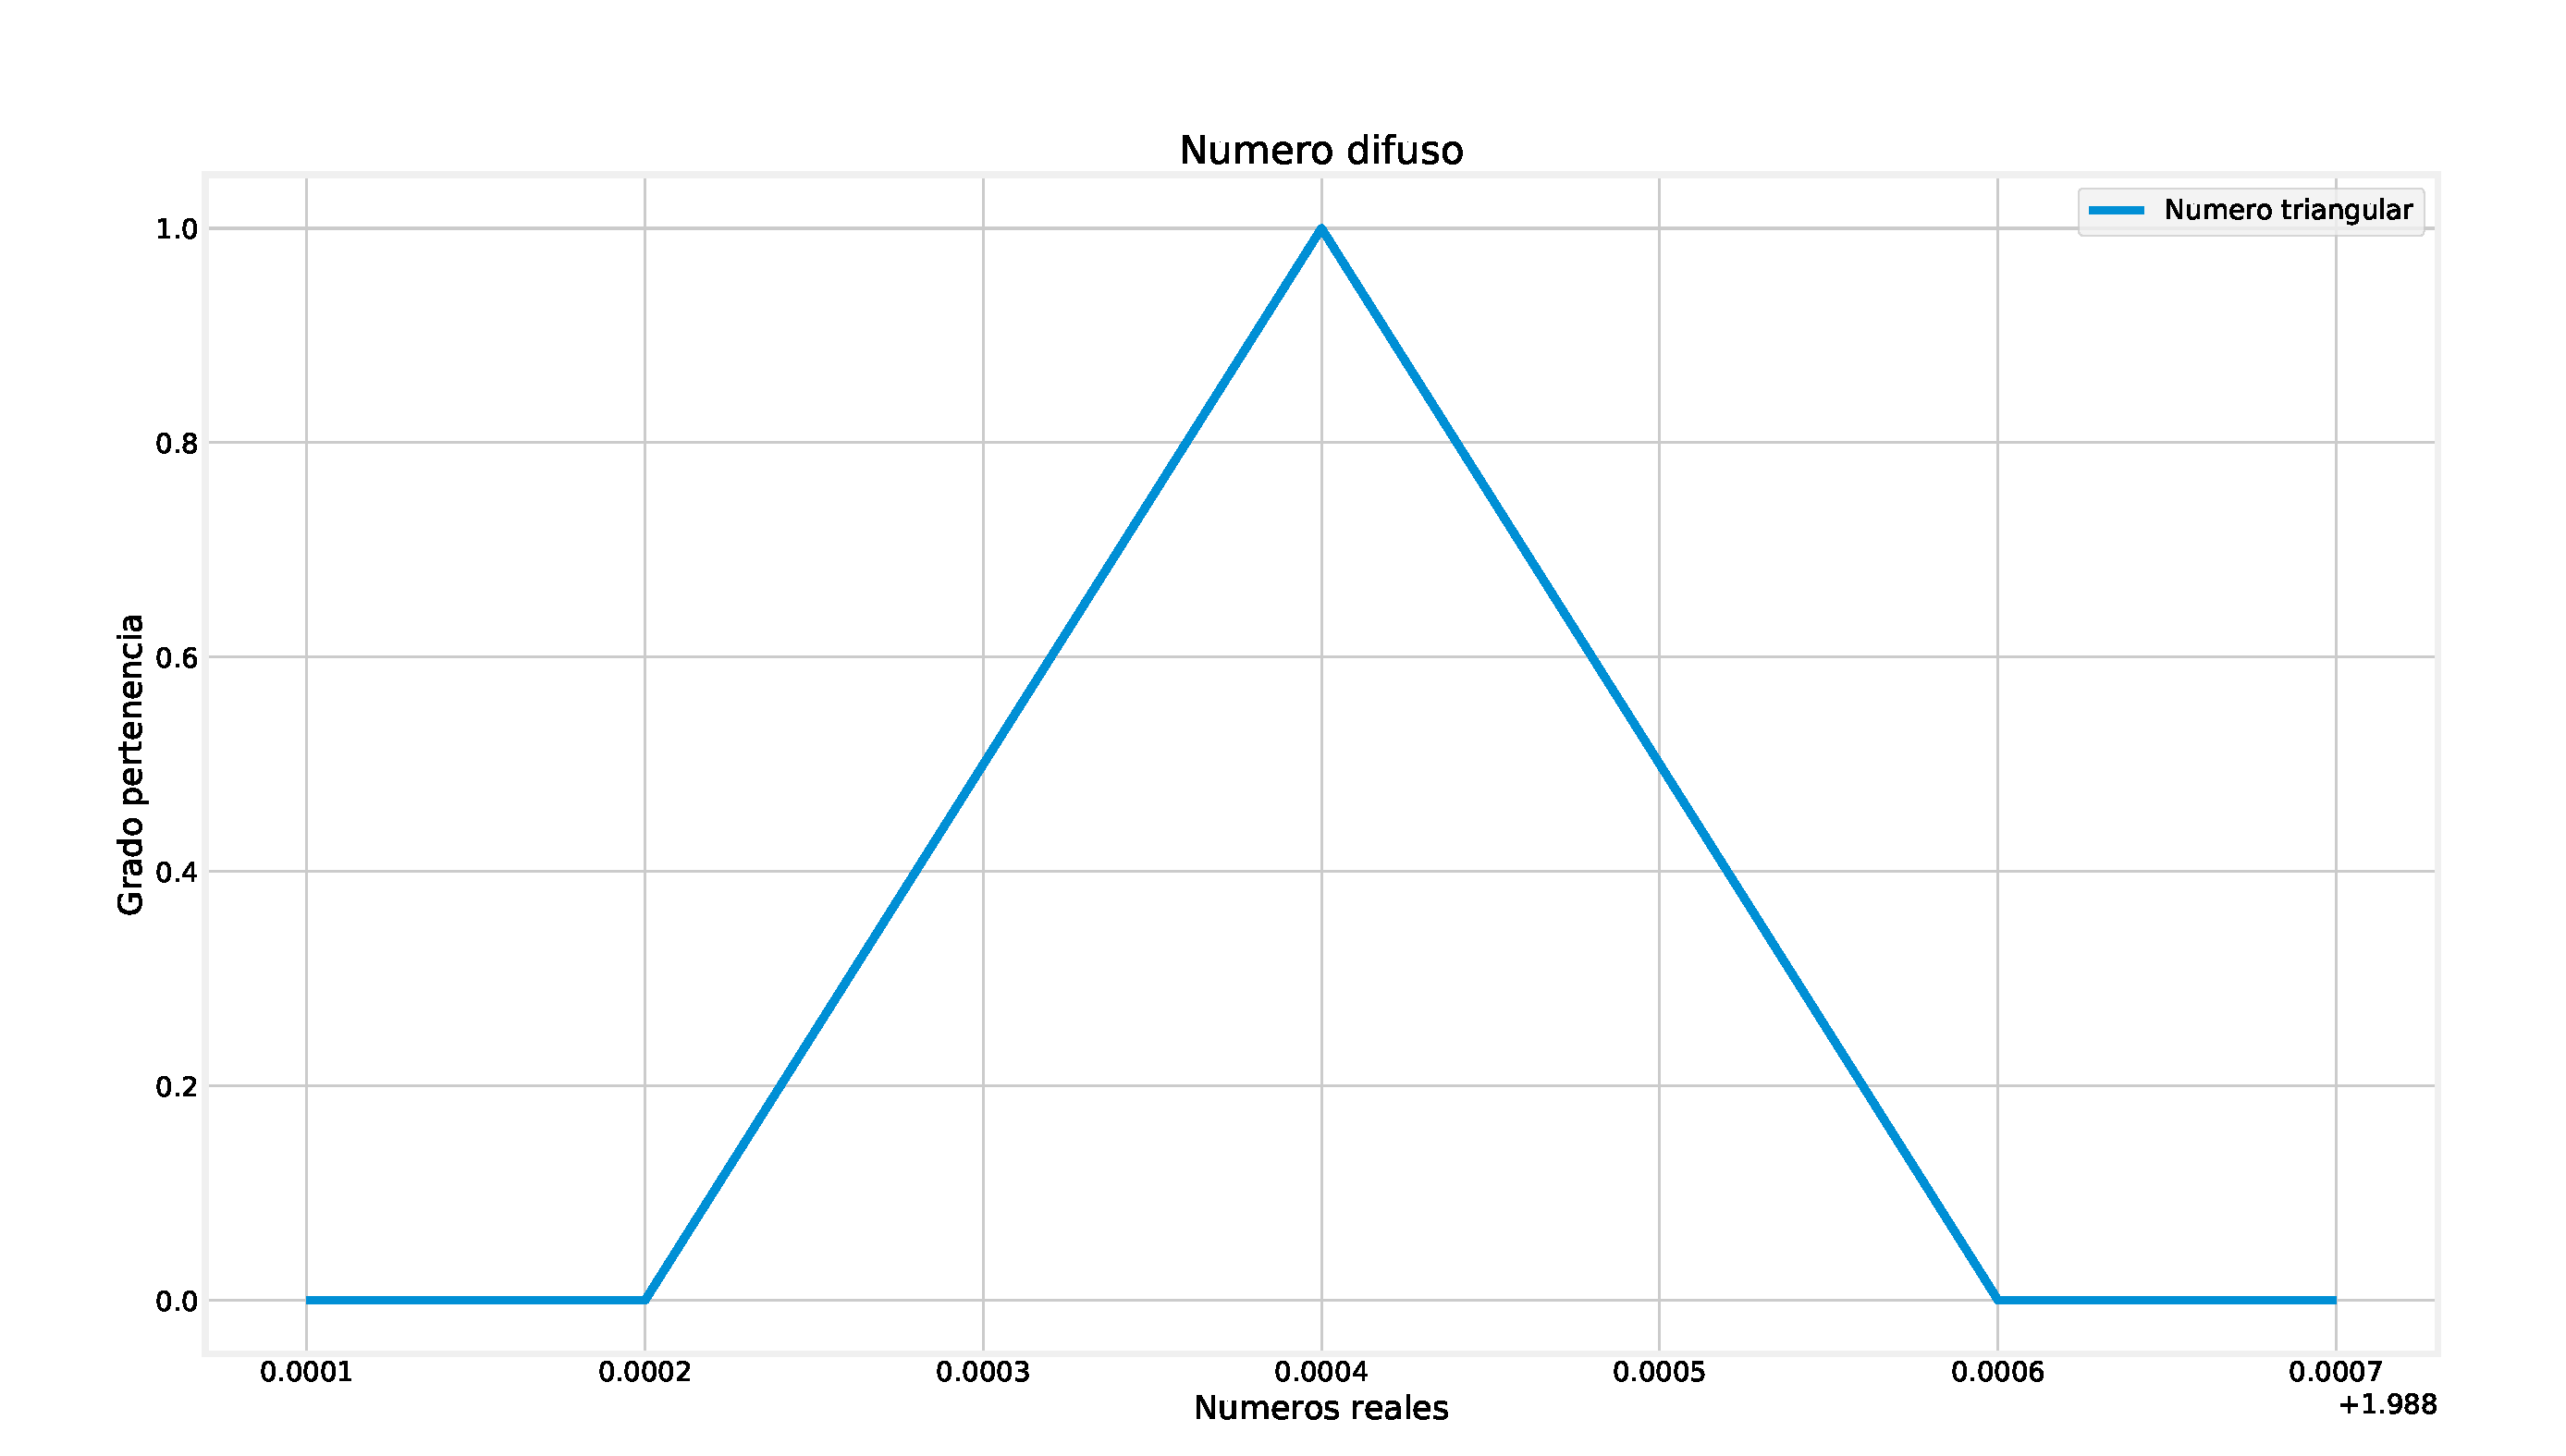
\includegraphics[width=\textwidth]{grafica_triangular_orbita_m.pdf}}
			\caption{Gráfica del número difuso $M$}
			\label{fig:triangular_m}
		\end{subfigure}
	\end{figure}
	
	Se puede observar también que tanto $a_x, a_y$ son funciones de clase $C^\infty$ en el abierto $\IR^2 - (0, 0)$, por tanto existe unicidad de soluciones (Teorema de Picard) y además, se puede aplicar el \hyperref[teorema:equivalencia]{Teorema de equivalencia entre EDO y EDD}, por tanto, se puede resolver este problema usando el método de Runge Kutta (Se verá en el último capítulo la resolución numérica de este problema)
	
\end{ejemplo}

\subsection{Aplicaciones a la mecánica cuántica}

% http://cds.cern.ch/record/518511/files/0107054.pdf
\subsection{Aplicaciones a reacciones químicas}
\subsection{Aplicaciones a la biología}

\section{Aplicaciones a las ciencias sociales}

\subsection{Aplicaciones a la economía}

\subsection{Aplicaciones a crecimientos de población}